\documentclass[times, utf8, seminar, numeric]{fer}
\usepackage{booktabs}
\usepackage{url}
\usepackage{rotating}
\usepackage{amsmath}

\begin{document}



% Ukljuci literaturu u seminar
\nocite{*}

% TODO: Navedite naslov rada.
\title{Naslov seminarskog rada}

% TODO: Navedite vaše ime i prezime.
\author{Ivan Katanić, Gustav Matula}

\voditelj{Mile Šikić}

\maketitle

\tableofcontents

\chapter{Uvod}
Mjere udaljenosti stringova od velike su važnosti u bioinformatici.
Najpoznatiji primjeri uključuju, Levenshteinovu (odnosno edit)
udaljenost i $LCS$ (longest common subsequence), odnosno najdulji
zajednički podniz.

Obje udaljenosti za dva stringa $a$ i $b$ u općenitom se slučaju
računaju dinamičkim programiranjem u složenosti $O(|a||b|)$, što ih,
usprkos sofisticiranim optimizacijama kako memorije, tako i vremena
izvođenja, nepraktičnim za velike primjere.

Zbog toga su razvijene modifikacije problema koje daju rjeđe matrice
dinamičkog programiranja i time omogućuju implementaciju koja je 
dovoljno efikasna na primjerima iz stvarnoga svijeta.

Primjer takve modifikacije je $LCS_k$ \cite{Benson}, koja zahtijeva da
se zajednički podniz sastoji od ne-preklapajućih podstringova
zadane duljine $k$. Jasno je da povećanjem $k$ dobivamo manji
broj parova jednakih podstringova dvaju stringova. S druge strane
za prevelik $k$ udaljenost je nula i mjera postaje beskorisna.

Mjera kojom smo se bavili u okviru ovog projekta je $LCS_{k++}$
\cite{Pavetic}, koja relaksira uvjet $LCS_k$ tako što dozvoljava
preklapanja. Drugim riječima, u $LCS_{k++}$ razmatraju se zajednički
podnizovi sastavljeni od podstringova duljine \textbf{barem} $k$.

Uzmimo za primjer stringove $a$ = "ABBABDCDAD" i $b$ = "BCBABBDCDBAD".
$LCS_{2++}(a,b) = 8$, podstring je "ABBDCDAD"
("\textbf{ABB}AB\textbf{DCDAD}", "BCB\textbf{ABBDCD}B\textbf{AD}").
$LCS_{3++}(a,b) = 6$, podstring je "ABBDCD"
("\textbf{ABB}AB\textbf{DCD}AD", "BCB\textbf{ABBDCD}BAD").

\chapter{Opis algoritma}

\section{Traženje \emph{točaka}}
Originalni $LCS_{k++}$ algoritam iz \cite{Pavetic}, kao  i neki
drugi $LCS$ algoritmi, kao početni korak traže sve parove indeksa $(i,
j)$ na kojima se ulazni par stringova ($a$, $b$) "poklapa". U
kontekstu običnog $LCS$-a, radi se o točkama za koje $a[i] = b[j]$.  U
kontekstu $LCS_k$, ili $LCS_{k++}$ promatramo točke za koje $a[i..i+k-1] =
b[j..j+k-1]$, odnosno za koje su podstringovi duljine $k$ koji počinju
na pripadajućim pozicijama jednaki. $LCS_k$ i $LCS_{k++}$ se naravno svode
na $LCS$ u slučaju $k = 1$. U nastavku ćemo se fokusirati na ovu drugu
definiciju, te ćemo parove koji je zadovoljavaju zvati jednostavno
\emph{točkama}, a njihove elemente \emph{koordinatama}.

Općenito rješenje ovog koraka moguće je napraviti u složenosti
$O(|a| + |b| + |r|)$ gdje je $|r|$ ukupan broj točaka \cite{poljaci}.
Ideja je konstruirati sufiksno polje nad stringom $a\#b$, te ga
podijeliti na segmente s $LCP >= k$. Unutar takvog segmenta svaki
par sufiksa gdje jedan dolazi iz $a$, a jedan iz $b$, definira jednu
točku. Uz odgovarajuća preslagivanja sufiksa unutar segmenata moguće
je točke generirati u redoslijedu rastuće prve, pa druge koordinate.

Ovaj pristup, iako teoretski zadovoljavajuć (složenost je optimalna),
u praksi se ne ponaša toliko dobro. Slijedeći \cite{Pavetic},
fokusirali smo se na manje vrijednosti $k$, za koje
je moguće napraviti savršeno sažimanje (\emph{perfect hashing}) u
64-bitne riječi. U cilju poboljšanja efikasnosti uveli smo neke
\emph{low-level} optimizacije. Tako primjerice za $k$ do $20$ i abecedu
do $4$ elementa, podstring od $k$ znakova možemo zapisati u $40$
bitova.  U preostalih $24$ bita možemo pohraniti indeks i oznaku
stringa iz kojeg podstring dolazi. Sortiranje niza cijelih brojeva
moguće je izvesti puno efikasnije od najbržih algoritama za
sortiranje sufiksa. Za to smo koristili vlastitu eksperimentalno 
optimiranu varijantu \emph{radix sorta}.

{opis tog sorta? detalji? jel treba uopće????????????????}

Nakon sortiranja algoritam je sličan prethodnom, niz (u ovom slučaju
podstringova, a ne sufiksa), dijeli se na segmente prema jednakosti,
te se iz odgovarajućih parova unutar segmenta generiraju točke.

Na primjer, za stringove $a =$ "ABC" i $c =$ "DAB" i $k = 2$
sortiranjem bi dobili niz $[(AB, a, 1), (AB, b, 2), (BC, a, 2), (DA,
  b, 1)]$, gdje trojke označavaju (\emph{podstring}, \emph{izvorni
  string}, \emph{indeks u izvornom stringu}). U tom primjeru imali
bi samo jedan zanimljiv segment, onaj za "AB", i iz njega bismo
generirali točku $(1, 2)$.

Valja napomenuti da u slučaju malog broja točaka ovaj dio algoritma
vremenski potpuno dominira nad ostatkom, te je dobar dio napora uložen
kako bi se toliko ubrzao (više o samom ubrzanju u kasnijem poglavlju).

\section{Traženje $LCS_{k++}$ iz točaka}
Preostaje iz već poznatih točaka pronaći sam $LCS_{k++}$. Ako s $P$
označimo skup točaka konstruiran u prethodnom koraku, rekurzivna
relacija dinamičkog programiranja na tako prorijeđenoj matrici ima
sljedeći oblik iz \cite{Pavetic}:

%% {dp relacija za sparse}
%% {
%%   za (i, j) iz P:
%%   dp(i, j) = max {
%%     (1)     k + max_{i' <= i - k, j' <= j - k}\{dp(i', j')\},
%%     (2)     1 + dp(i-1, j-1) ako (i-1, j-1) \in P
%%   }
%% }

\begin{align*}
dp(i, j) = \max\{ \\
  &k + \max_{i' \le i - k, j' \le j - k}\{dp(i', j')\},    &      (1) \\ 
  &1 + dp(i-1, j-1) \text{, ako } (i-1, j-1) \in P     &       (2)\\
  \}
\end{align*}

Ako imamo niz $V$ točaka koji sadrži točke iz $P$ sortirane po prvoj,
pa po drugoj koordinati, lako je za svaku točku $(i, j)$ pronaći
indeks točke $(i-1, j-1)$, u slučaju da je prisutna u nizu. To možemo
napraviti u amortizirano linearnom vremenu jednim prolaskom kroz niz
$V$, i time je dio (2) riješen. U \cite{Pavetic} isto je izvedeno
binarnim pretraživanjem, što je neznatno sporije. Ako točke $(i, j)$ i
$(i-1, j-1)$ postoje, kažemo da je druga \emph{nastavak} prve.

Dio (2) je nešto složeniji. U \cite{Pavetic} koristi se prolaz po retcima
pa po stupcima (u smislu koordinata točaka), pri čemu se održava
struktura podataka (Fenwickovo stablo) koja omogućuje računanje gornjeg
maksimuma u logaritamskoj složenosti. 

Naš pristup vođen je idejom algoritma za $LCS$ iz \cite{Hunt}, koju je uz neke
manje trivijalne opservacije moguće prilagoditi za $LCS_{k++}$. Za početak
ćemo objasniti ideju za $LCS$, a onda i proširenje na $LCS_{k++}$.

\subsection{Huntov algoritam}
U radu Hunta i Szymanskog (\cite{Hunt}) također se radi prolaz po
retcima pa po stupcima. Glavna ideja iz je (po opisu iz \cite{Survey})
održavati niz $MinYPos[l]$, koji uz pretpostavku da smo trenutno u
retku $i$ označava minimalni $j$ takav da je $LCS(a[1..i], b[1..j]) =
l$. Primijetimo da je $MinYPos$ nužno rastući niz.

Pretpostavimo da smo obradili točke $(i', j')$ s $i' < i$, te sada
promatramo točke $(i, j)$, za neki fiksni $i$. Pretpostavimo da
$MinYPos[l] < j$.  Tada postoji $LCS$ duljine $l$ koji završava točkom
$(i', j')$ gdje $i' < i$ i $j' < j$. Taj je $LCS$ moguće proširiti točkom
$(i, j)$, pa znamo da nakon obrade trenutnog retka mora vrijediti
$MinYPos[l+1] <= j$.  

Vidimo da je dovoljno pronaći $l$ takav da $MinYPos[l] < j <=
MinYPos[l+1]$, što možemo napraviti binarnim pretraživanjem, te
postaviti $MinYPos[l+1]$ na $j$ (jer niz duljine $l$ koji završava
na $MinYPos[l]$ proširujemo u niz duljine $l+1$ koji završava na
$j$).

Ovdje treba napomenuti da je redoslijed obilaska točaka za fiksni $i$
bitan. Točke treba obići padajuće po stupcima, kako bi se promjene
niza $MinYPos$ dogodile efektivno paralelno. U protivnom se može
dogoditi da izgradimo ilegalan $LCS$ koji sadrži točke u istom
retku.

\subsection{Kuoov algoritam}
Huntov algoritam pojednostavljen je u \cite{Kuo} tako da se umijesto
binarnog pretraživanja radi amortizirano linearan prolaz po trenutnom
retku i nizu $MinYPrefix$. Dakle dok prolazimo kroz točke u trenutng 
retka, ujedno održavamo odgovarajući indeks $l$ u $MinYPrefix$, koji
za trenutnu točku $(i, j)$ povećavamo dok $MinYPrefix[l] < j$. 
Na prvi pogled to pogoršava složenost algoritma. Taj instinkt je
točan u općenitom slučaju, no svejedno analizirajmo detaljnije
složenosti tih dvaju pristupa.

Recimo da u trenutnom retku $i$ imamo $t$ točaka. Huntov algoritam
primijenjen na jednom retku ima složenost $O(t \log r)$, gdje je
$r$ najdulji $LCS$ koji smo do sad pronašli. S druge strane algoritam
Kuoov algoritam ima složenost $O(t + r)$. Dakle jasno je da je za
veći $r$ bolji Huntov algoritam, a za manji Kuoov.

\subsection{Proširenje na $LCS_{k++}$}
Prvo ćemo malo modificirati značenje niza $MinYPrefix$.
Za algoritam koji slijedi $MinYPrefix[l]$ označava najmanji $j$
takav da $LCS_{k++}(a[1..i+k-1], b[1..j+k-1]) >= l$. Razlika je
u tome što smo znak jednakosti zamijenili u znak nejednakosti
(promijenili smo i intervale da uzmemo u obzir duljinu $k$). 
Ta promjena je ključna za očuvanje važnog svojstva $MinYPrefix$:
niz mora biti ne-padajući kako bismo ga mogli binarno pretraživati.

Kako bismo se uvjerili u nužnost uvjeta, zamislimo instancu u kojoj
nema nastavaka (dakle ako postoji točka $(i, j)$, tada ne postoji
$(i-1, j-1)$). U tom slučaju $MinYPrefix[l]$ može biti veći od
nule samo za $l$ djeljiv s $k$. Za $k > 1$ takav niz će rijetko
biti ne-padajuć.

Tijekom obrade točaka iz retka $i$, potreban nam je $MinYPrefix$ u
stanju u kojem je bio nakon obrade retka $i-k$, pa zasad
jednostavno pretpostavimo da nam je dostupan. Označimo ga s
$MinYPrefix_{i-k}$. Promatramo točku $(i, j)$. Ona se može
nastaviti na$ LCS_{k++}$ koji završava u točki $(i', j')$ s $i' <=
i - k$ i $j' <= j - k$. Po gornjoj pretpostavci točke uračunate u
$MinYPrefix$ zadovoljavaju prvu nejednakost. Za drugu, slično kao
u Huntovom, odnosno Kuoovom algoritmu, pronađemo $l$ takav da
$MinYPrefix[l] < j - k + 1 <= MinYPrefix[l+1]$. Tada znamo da
postoji $LCS_{k++}$ duljine $l$ koji se točkom $(i, j)$ može
proširiti u $LCS_{k++}$ duljine $l+k$. Štoviše, u koliko $(i, j)$
nema nastavak, znamo da je $dp(i, j) = l+k$.  Ako ipak postoji,
$dp(i, j) = max\{l+k, 1+dp(i-1, j-1)\}$. Time smo izračunali
vrijednosti tablice dinamičkog programiranja u svim točkama
$i$-tog retka. Konačan algoritam bira između Huntovog i Kuoovog
pristupa jednostavnom procjene vremena izvršavanja temeljene na
njihovim teorijskim složenostima i empirijski utvrđenoj konstanti.

Zatim moramo modificirati $MinYPrefix$ uzevši u obzir rezultate
$i$-tog retka. U slučaju da $dp(i, j) = dp(i-1,j-1)+1$,
jednostavno postavimo $MinYPrefix_i[dp(i,j)] =
min\{MinYPrefix_{i-1}[dp(i,j)], j\}$.  Inače $dp(i, j) = l+k$, te
postavljamo $MinYPrefix_i[l+s] = min\{MinYPrefix_{i-1}[l+s], j\}$
za sve $s$ iz $[1..k]$. Prvi instinkt je uzeti samo $s = k$, ali
po gornjoj redefiniciji $MinYPrefix$, to nije dovoljno. Znamo da
$MinYPrefix_{i-1}[l+s] <= j$, za $s$ iz $[-l..0]$, budući da
$MinYPrefix_{i-k}[l+s] <= j$ za $s$ iz istog intervala (slijedi iz
definicije $l$ i činjenice da vrijednosti $MinYPrefix$ za fiksni
indeks ne mogu rasti). Ali moguće je na primjer da
$MinYPrefix_{i-1}[l+k-1] > j$ (naravno uz pretpostavku $k > 1$).
Ali budući da točkom u stupcu $j$ možemo dobiti $LCS_{k++}$ duljine
$l+k$, i $l+k >= l+k-1$, mora vrijediti $MinYPrefix_i[l+k-1] <= j$.
Analogan argument vrijedi za ostale $s$ iz $[1..k-1]$.

Za kraj preostaje objasniti kako dobiti $MinYPrefix_{i-k}$.
Najjednostavnije je podijeliti obradu retka na računanje
vrijednosti tablice dinamičkog programiranja i osvježavanje niza
$MinYPrefix$. Tako nakon što osvježimo $MinYPrefix$ za redak
$i-k$, možemo odmah izračunati $dp$ za redak $i$. A kad dođemo do
retka $i$, prvo osvježimo $MinYPrefix$, a zatim računamo $dp$ za
redak $i+k$ (ako takav postoji), i tako dalje.

\chapter{Rezultati}
Zadatak je bio dobiti implementaciju barem tri puta bržu od
originalnog $LCS_{k++}$ \cite{github}. Brzinu rješenja testirali
smo na stringovima duljine $n = 10000$ (za veći $n$ faktor ubrzanja
našeg algoritma još je veći), s abecedom od četiri znaka, za $k$ od
$4$ do $20$. Probabilistički model ulaznih stringova za testiranje
preuzeli smo iz \cite{Pavetic}. Tako smo prvi string generirali iz
uniformne distribucije svih stringova duljine $n$, a drugi iz prvog
uz zadanu sličnost $p$ (za svaki znak bi s vjerojatnošću $p$ uzeli
isti znak kao u prvom stringu, a s vjerojatnošću $1-p$ uniformno
jedan od preostalih znakova.

Sljedeći graf prikazuje faktore ubrzanja postignute za različite
vrijednosti $k$ i različite sličnosti stringova. 

\begin{sidewaysfigure}[p]
  \begin{center}
    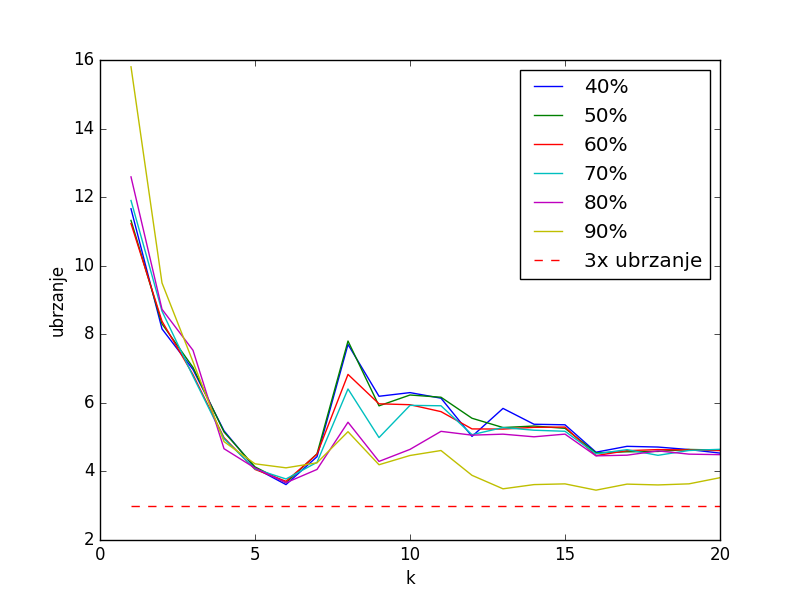
\includegraphics{../../test/speedplot.png}
  \end{center}
  \centering
  \textbf{Slika 1.1}  
\end{sidewaysfigure}

Kako bismo dobili što stabilnije rezultate, za svaki par stringova
oba smo algoritma pokrenuli $30$ puta, i zatim uzeli omjer ukupnih
vremena izvršavanja. Testiranje je izvedeno na {Kaletov procesor i
  što već}.

U zadatku nije bilo posebnih zahtjeva što se tiče memorije, svejedno
na primjerima na koje smo ručno otprilike provjerili naš je
algoritam koristio manje memorije od originala (konkretno mjerili
smo virtualnu memoriju alatom ps).


\chapter{Zaključak}
Vidjeli smo da se poopćenjem poznatih $LCS$ algoritama može 
računati $LCS_{k++}$ na način dosta drukčiji od onog u originalu.
Uz \emph{low-level} optimizacije postigli više nego trostruko ubrzanje
nad originalnom implementacijom.

Prostora za dodatna ubrzanja još svakako ima. Najbolji omjer ubrzanja
i uloženog truda sigurno bi dalo iskorištavanje paralelizam modernih
procesora, zatim istraživanje alternativnih algoritama, te konačno
dodatne \emph{low-level} optimizacije našeg algoritma.

\bibliography{literatura}
\bibliographystyle{fer}

\end{document}
